%%%%%%%%%%%%%%%%%%%%%%%%%%%%%%%%%%%%%%%%%
% Journal Article
% LaTeX Template
% Version 1.3 (9/9/13)
%
% This template has been downloaded from:
% http://www.LaTeXTemplates.com
%
% Original author:
% Frits Wenneker (http://www.howtotex.com)
%
% License:
% CC BY-NC-SA 3.0 (http://creativecommons.org/licenses/by-nc-sa/3.0/)
%
%%%%%%%%%%%%%%%%%%%%%%%%%%%%%%%%%%%%%%%%%

%----------------------------------------------------------------------------------------
%	PACKAGES AND OTHER DOCUMENT CONFIGURATIONS
%----------------------------------------------------------------------------------------

\documentclass{article}

%\documentclass{aastex}  % version 5.0 or prior
%\usepackage{natbib}



\usepackage{graphicx}
\usepackage{lipsum} % Package to generate dummy text throughout this template
%\usepackage[sc]{mathpazo} % Use the Palatino font
\usepackage[T1]{fontenc} % Use 8-bit encoding that has 256 glyphs
\linespread{1.05} % Line spacing - Palatino needs more space between lines
\usepackage{microtype} % Slightly tweak font spacing for aesthetics

\usepackage[margin=1in,columnsep=20pt]{geometry} % Document margins
\usepackage{multicol} % Used for the two-column layout of the document
\usepackage[hang, small,labelfont=bf,up,textfont=it,up]{caption} % Custom captions under/above floats in tables or figures
\usepackage{booktabs} % Horizontal rules in tables
\usepackage{float} % Required for tables and figures in the multi-column environment - they need to be placed in specific locations with the [H] (e.g. \begin{table}[H])
\usepackage{hyperref} % For hyperlinks in the PDF
\usepackage{subcaption}

\usepackage{lettrine} % The lettrine is the first enlarged letter at the beginning of the text
\usepackage{paralist} % Used for the compactitem environment which makes bullet points with less space between them
\usepackage{amsmath}
\usepackage{abstract} % Allows abstract customization
\renewcommand{\abstractnamefont}{\normalfont\bfseries} % Set the "Abstract" text to bold
\renewcommand{\abstracttextfont}{\normalfont\small\itshape} % Set the abstract itself to small italic text

\usepackage{titlesec} % Allows customization of titles
%\renewcommand\thesection{\Roman{section}} % Roman numerals for the sections
%\renewcommand\thesubsection{\Roman{subsection}} % Roman numerals for subsections
%\renewcommand\thesubsubsection{\Alph{subsubsection}} % Roman numerals for subsections
\titleformat{\section}[block]{\Large\scshape}{\thesection}{1em}{} % Change the look of the section titles
\titleformat{\subsection}[block]{\large}{\thesubsection}{1em}{} % Change the look of the section titles
\titleformat{\subsubsection}[block]{}{\thesubsubsection}{1em}{} % Change the look of the section titles

\usepackage{fancyhdr} % Headers and footers
\pagestyle{fancy} % All pages have headers and footers
\fancyhead{} % Blank out the default header
\fancyfoot{} % Blank out the default footer
\fancyhead[C]{Montana State University \quad $\bullet$ \quad CSCI 466 Artificial Intelligence \quad $\bullet$ \quad Group 21} % Custom header text
\fancyfoot[RO,LE]{\thepage} % Custom footer text

\newcommand{\ve}[1]{\boldsymbol{\mathbf{#1}}}

%----------------------------------------------------------------------------------------
%	TITLE SECTION
%----------------------------------------------------------------------------------------

\title{\vspace{-15mm}\fontsize{24pt}{10pt}\selectfont\textbf{CSCI 446 Artificial Intelligence \\ Project 1 Final Report} \\[-2mm]} % Article title
\date{\today}
\author{
\large
\textsc{Roy Smart} \and \textsc{Nevin Leh} \and \textsc{Brian Marsh}\\[2mm] % Your name
}


%----------------------------------------------------------------------------------------

\begin{document}

\maketitle % Insert title

\thispagestyle{fancy} % All pages have headers and footers

%\begin{abstract}
%We present a novel way of performing MOSES data inversions using a
%\end{abstract}

%----------------------------------------------------------------------------------------
%	ARTICLE CONTENTS
%----------------------------------------------------------------------------------------

%\begin{multicols}{2} % Two-column layout throughout the main article text
\normalsize

\begin{abstract}
	Our project aims to find solutions to the Graph Coloring Problem by using five different algorithms and comparing their performance.  The algorithms used are Minimum Conflicts, Simple Backtracking, Backtracking with Forward Checking, Backtracking with Constraint Propagation, and Local Search using a Genetic Algorithm.  We studied their read, write, and function call counts to measure performance.  The time that each algorithm takes to find a solution is used as a secondary metric, but is understood to be inconsistent as a result of involving many variables.  Our project found that the Minimum Conflicts performed the best in general, but that Local Search using a Genetic Algorithm also performed well with the potential for exceeding the other’s performances for larger variations of the problem.  Further study would be needed to investigate this hypothesis, which is beyond the scope of this project.
\end{abstract}
\section{Introduction}
	The \textit{Graph Coloring Problem} (GCP) is the problem of attempting to color a set of interconnected vertices, using a limited set of colors, such that no vertex has the same color as its neighbors. This problem is best visualized as the map coloring problem. As an example of the map coloring problem, consider the problem of assigning one of four colors to every country in the world, such that no two adjacent countries have the same color, as in Figure \ref{world}. 
	\begin{figure}[h!]
		\centering
		\includegraphics[width=0.8\textwidth]{images/world_map}
		\caption{Map of the world satisfying the map coloring problem \cite{world}.}
		\label{world}
	\end{figure}
	It can be shown that the map coloring problem reduces to the graph coloring problem\cite{ai} if we represent the countires as the vertices of the graph and the borders between countries as the edges of the graph, shown in Figure \ref{four_col}. This configuration produces a graph with no edge intersections, called a \textit{planar} graph. 	
	\begin{figure}[h!]
		\centering
		\includegraphics[width=0.6\textwidth]{images/four_color}
		\caption{Diagram describing how the map coloring problem can be transformed into the graph coloring problem \cite{four_color}.}
		\label{four_col}
	\end{figure}
	For this project, we are asked to solve the GCP problem for planar graphs only. Since the problems are guaranteed to be planar, we will represent our graphs using polygon maps generated by our program.
	
	To solve the GCP we employed five different algorithms: Minimum Conflicts, Simple Backtracking, Backtracking with Forward Checking, Backtracking with Constraint Propagation (MAC), and Local Search using a Genetic Algorithm. To evaluate these algorithms, we built a problem generating program that can produce a random set of planar graphs. Using the problem generator, we calculated a set of graphs between the sizes \{10, 20, 30,...,100\} and called the five graph coloring algorithms to solve the GCP. We measured GCP algorithm performance by measuring the number of read/write operations, the time required to find a solution, and the number of function calls for each algorithm. Using these metrics, we predict that the Minimum Conflicts algorithm will be the fastest, based off its performance on the eight-queens problem\cite{MINTON}.


\par The code for this project is implemented in \texttt{C++} and depends on the programs \texttt{cairo}, \texttt{gnuplot}, \texttt{ffmpeg}, and \LaTeX \space for graph output, performance output, video output, and documentation respectively.


\section{Problem Generation}
	We created a function that could produce many examples of planar graphs from a set of randomly scattered points. For an arbitrary set of points, there is no unique planar graph that can be constructed. To solve this issue, the problem statement has provided an algorithm for calculating an planar graph. 
	\begin{quote}
	Select some point $X$ at random and connect $X$ by a straight line
	to the nearest point $Y$ such that $X$ is not already connected to $Y$ and the line crosses no other line. Repeat the
	previous step until no more connections are possible.
	\end{quote}
	For our implementation of the above algorithm, we started by creating a complete graph (where each vertex is connected to every other vertex). Each vertex was associated with a list of edges, sorted by length. 
	We then selected a point at random and inspected the first unchecked edge $E$. If $E$ did not cross any of the accepted edges, it was added to the list of accepted edges and marked as checked. This process was repeated until every edge was marked as checked. \par
	The most challenging part of the implementation described above was determining if two line segments intersected. An algorithm to determine if two edges (or line segments) cross has been outlined by LaMothe \cite{tricks} and described in detail here. Let us start by defining two line segments 
	\begin{align}
		\begin{split}
			& A = \{ \ve{a},\; \ve{a'} \} \\
			& B = \{\ve{b}, \;\ve{b'}\}
		\end{split}
	\end{align}
	where $\ve{a}, \; \ve{a'}, \; \ve{b}, \text{ and } \ve{b'}$ are vectors from the origin to the ends of the line segments. Next, compute the direction vectors for each line segment
	\begin{align}
		\begin{split}
			&\ve{\alpha} = \ve{a}' - \ve{a} \\
			&\ve{\beta} = \ve{b}' - \ve{b} 
		\end{split}
	\end{align}
	Now, the trick to solving this problem is to parameterize the line segment using the direction vector and a parameter $t_i$ in the domain $[0, \; 1]$.
	\begin{align}
		\begin{split}
			& \ve{p} = \ve{a} + \ve{\alpha} t_a, \quad t_a \in [0, \; 1]\\
			& \ve{q} = \ve{b} + \ve{\beta} t_b, \quad t_b \in [0, \; 1]
		\end{split}
	\end{align}
	From here, the solution is obvious. To find the point of intersection, we set $\ve{p} = \ve{q}$ and solve for the values of $t_a$ and $t_b$. Then, if the solution is outside the domain of $t_i$, the line segments do not intersect. Thus,
	\begin{align}
		\Rightarrow \; &\begin{cases}
			p_x = q_x \\
			p_y = q_y
		\end{cases} \\
		\Rightarrow \; & \begin{cases}
			a_x + \alpha_x t_a = b_x + \beta_x t_b \\
			a_y + \alpha_y t_a = b_y + \beta_y t_b.
		\end{cases} \label{system}	
	\end{align}
	Equation \ref{system} is a system of two equations and two unknowns, solving for $t_a$ and $t_b$ gives
	\begin{align}
		\begin{split}
			&t_a = \frac{(-a_y + b_y)\beta_x + (a_x - b_x)\beta_y}{\alpha_y \beta_x - \alpha_x \beta_y} \\
			&t_b = \frac{(a_y - b_y)\alpha_x + (-a_x + b_x)\alpha_y}{-\alpha_y \beta_x + \alpha_x \beta_y}.
		\end{split} \label{final_expr}
	\end{align}
	Finally, we can determine whether $A$ and $B$ intersect if $0 < t_a < 1$ and $0 < t_b < 1$ evaluates to true. This method may be more inefficient than other algorithms, such as the example outlined by Cormen\cite{structs} due to the division operation in Equation \ref{final_expr}. \par 
	Using the expression above to determine line intersections, we were able to implement a problem generator that was reasonably efficient, generating approximately $1\times10^3$ examples per second. This efficiency was important, because it made testing and debugging the GCP algorithms much faster. Example output from the problem generator is shown in Figure \ref{pgen}.
	
	\begin{figure}[h!]
		\centering
		\begin{subfigure}{0.45\textwidth}
			\centering
			\includegraphics[width=\textwidth]{images/pgen}
			\caption{Planar graph with 100 vertices.}
			\label{pgen}
		\end{subfigure}
		\qquad
		\begin{subfigure}{0.45\textwidth}
			\centering
				\includegraphics[width=\textwidth]{images/pgen_poly}
				\caption{Polygon map corresponding to (a).}
				\label{pgen_poly}
		\end{subfigure}
		\caption{Visualization of the output of the problem generator. First a planar graph was created (a), and then a corresponding polygon map was found (b).}
	\end{figure}
	
	We have also implemented a way to produce a map of regions that is analogous to the graphs created by the problem generator, shown in Figure \ref{pgen_poly}.  
	Since the graph coloring problem does not uniquely define the map coloring problem, we had to invent a metric that produces appropriate graphs. To define our metric, consider that if a polygon $G_i$ corresponding to each point $P_i$ was constructed out of the midpoints $M_{i,m}$ of the associated edges $E_{i,m}$ of $P_i$, then an adjacent polygon $G_j$ would only touch at the corners. This would cause our map to be full of gaps. Therefore, to fix the problem we also define the centroid $C_{i,n}$ of each triangle $T_{i,n}$ formed by the two adjacent edges $E_{i,m}$ and $E_{i,m+1}$. We then define the final polygon for $P_i$ using the points $M_{i,m}$ and $C_{i,n}$. This procedure is unnecessary in terms of the assignment, but is helpful for debugging GCP algorithms and demonstrating example output, as well as for aesthetic pleasure.
		
\section{Minimum Conflicts}
	\subsection{Description}
		
		Minimum conflicts uses a relatively simple algorithm to solve constraint satisfaction problems.  A step towards solving the problem is made based upon how many conflicts a variable has with other variables.  As it runs, the algorithm updates the number of conflicts until none remain for any of the variables, meaning the problem is solved, or a time limit is reached, in which no solution is found.
		
		The implementation of minimum conflicts for the graph coloring problem begins by coloring the graph at random.  Each node of the graph is given a conflict score to represent how many conflicts it has with its neighbors.  The algorithm starts by randomly selecting a node with conflicts and changing it to a color that will result in the minimal conflict score.  The affected nodes update their conflict scores and the process repeats until no conflicts remain.

				
		\begin{figure}[h!]
			\begin{subfigure}{0.18\textwidth}
				\centering
				\includegraphics[width=\textwidth]{images/sequences/min/minconf_I00003}
				\caption{}
				\label{mina}
			\end{subfigure}
			\;
			\begin{subfigure}{0.18\textwidth}
				\centering
				\includegraphics[width=\textwidth]{images/sequences/min/minconf_I00004}
				\caption{}
				\label{minb}
			\end{subfigure}
			\;
			\begin{subfigure}{0.18\textwidth}
				\centering
				\includegraphics[width=\textwidth]{images/sequences/min/minconf_I00005}
				\caption{}
				\label{minc}
			\end{subfigure}
			\;
			\begin{subfigure}{0.18\textwidth}
				\centering
				\includegraphics[width=\textwidth]{images/sequences/min/minconf_I00006}
				\caption{}
				\label{mind}
			\end{subfigure}
			\;
			\begin{subfigure}{0.18\textwidth}
				\centering
				\includegraphics[width=\textwidth]{images/sequences/min/minconf_I00007}
				\caption{}
				\label{mine}
			\end{subfigure} 

			\caption{A map coloring example using minimum conflicts on a graph with 10 vertices.}
			\label{min_ex}
		\end{figure}


		Figure \ref{min_ex} provides an example of minimum conflicts to better describe the steps it takes.  The first image is a randomly colored graph in which $N = 8$. An easy to see example is the transition from \ref{mind} to \ref{mine}.  The algorithm randomly selects a node with conflicts, the blue node at the top of the panel, and considers all of the possible colors it could be changed to. This node has a conflict because it borders another blue node.   The color with the lowest conflict score, green, is selected and the node is changed to this color. Green was selected because the node already bordered a red, pink, and red region. The result is a correctly colored graph. If there were more conflicts, the process would repeat until the graph did not have any more conflicts.  
		
		Although this sequence of pictures shows an efficient solution to the graph coloring problem, the majority of the work done by this algorithm takes place behind the scenes.  Before the color of each node is selected, it must be compared to the colors of each of the neighboring nodes.  For a node with 5 neighbors, using a set of five colors, the minimum conflicts algorithm requires 25 reads for this single step.  This facet of the algorithm causes the mean number of reads to greatly exceed those of both writes and steps.

		Our implementation of the minimum conflicts algorithm is based upon Figure 6.8 in Russel and Norvig \cite{ai} which outlines the structure of a minimum conflicts algorithm. The result was  a \texttt{for} loop that ends upon a maximum number of steps being reached, unless a solution is found first.  The function returns \texttt{true} if it ends prematurely from the check \texttt{if (map->num\_conflicts() == 0)} is satisfied, which indicates a solution.  Otherwise, the function returns \texttt{false} if the maximum number of steps is reached and the \texttt{for} loop is completed, indicating that a solution was not found. At each iteration of the loop a conflicting node is chosen at random and is minimized.
		
		One important feature of our implementation was that, if every color caused the same number of conflicts, a random color was chosen for that vertex rather than keeping its original color. This kept the program from getting deadlocked in a situation where one vertex was depending on a second vertex that relies on a third vertex. If the third vertex is chosen but remains the same color it can keep the second vertex from changing color and, therefore, the first vertex is stuck. 
		
		

	\subsection{Experimental Approach}
	To gauge the performance of the algorithm we will run the algorithm on graph sizes $N = (10, 20, ..., 100)$ with 20 runs of each different graph size. From each run we saved the number of vertex reads, vertex writes, steps taken by the program. The number of steps was defined as the number of times a vertex was chosen to be minimized. This metric was useful for measuring backtracking against itself while the vertex reads and writes were good for comparing its performance to the other algorithms.
	
	
	\subsection{Results}
	
			\begin{figure}[h!]
				\centering
				\includegraphics[width=0.6\textwidth]{../results_5/min_conflicts/min_conflicts_performance}
				\caption{Logarithmic plot describing the performance of the min-conflicts algorithm vs. the number of vertices. The shaded regions represent the minimum and maximum values of each quantity.}
				\label{minconf}
			\end{figure}
			
	 Figure \ref{minconf} shows  that minimum conflicts ran in exponential time. While the lines are linear on the plot, the plot is logarithmic, implying that the exponent is increasing by some constant multiplied by $N$. An interesting point is that even though the algorithm is running in exponential time, it is much faster than brute force and faster than any of the other algorithms tested. This follows our expectations that stemmed from the fact that minimum conflicts is faster than backtracking when solving the eight-queens problem\cite{MINTON}.
	
	There are several interesting aspects of the plot that can be explained by the structure of our code. The first is that the number of vertex reads far outstrips number of steps and writes. This is due to the fact that in each step all of the chosen vertex's neighbors are read while only the vertex itself is written to.
	
	Another interesting aspect is that the number of vertex writes slightly exceeds the number of steps taken. This is explained by the fact that the algorithm actually has to write a color each time it checks that color for number of conflicts. Since the algorithm has to check four colors and then write a color the total number of writes per step is actually five.

\section{Simple Backtracking}
	\subsection{Description}
		\label{simpe_desc}
		Backtracking is a method of solving constraint satisfaction problems through an "educated" exhaustive search. It works by building a partial solution one component at a time and then testing the solution to check if the solution still has a chance of success \cite{Golomb}. If the solution cannot possibly succeed, the algorithm \textit{backtracks} by moving back one component, modifying the component to form a new partial solution and then continuing. By checking partial solutions, backtracking can eliminate large portions of the solution-space, thus yielding greater efficiency than a simple exhaustive search.
		
		In the graph coloring problem, backtracking assigns colors to one vertex at a time and checks to see if it has the same value as any of its neighbors. If none of the possible colors work for the current vertex, it backs up and tries a different color on a previously assigned vertex. If a color has no conflicts, backtracking continues to the next vertex in the sequence.
		
		\begin{figure}[h!]
			\begin{subfigure}{0.18\textwidth}
				\centering
				\includegraphics[width=\textwidth]{images/sequences/simple_backtracking/bt_simple_I00001}
				\caption{}
				\label{bta}
			\end{subfigure}
			\;
			\begin{subfigure}{0.18\textwidth}
				\centering
				\includegraphics[width=\textwidth]{images/sequences/simple_backtracking/bt_simple_I00002}
				\caption{}
				\label{btb}
			\end{subfigure}
			\;
			\begin{subfigure}{0.18\textwidth}
				\centering
				\includegraphics[width=\textwidth]{images/sequences/simple_backtracking/bt_simple_I00004}
				\caption{}
				\label{btc}
			\end{subfigure}
			\;
			\begin{subfigure}{0.18\textwidth}
				\centering
				\includegraphics[width=\textwidth]{images/sequences/simple_backtracking/bt_simple_I00006}
				\caption{}
				\label{btd}
			\end{subfigure}
			\;
			\begin{subfigure}{0.18\textwidth}
				\centering
				\includegraphics[width=\textwidth]{images/sequences/simple_backtracking/bt_simple_I00007}
				\caption{}
				\label{bte}
			\end{subfigure} \\
			
			\begin{subfigure}{0.18\textwidth}
				\centering
				\includegraphics[width=\textwidth]{images/sequences/simple_backtracking/bt_simple_I00009}
				\caption{}
				\label{bt1}
			\end{subfigure}
			\;
			\begin{subfigure}{0.18\textwidth}
				\centering
				\includegraphics[width=\textwidth]{images/sequences/simple_backtracking/bt_simple_I00012}
				\caption{}
				\label{bt2}
			\end{subfigure}
			\;
			\begin{subfigure}{0.18\textwidth}
				\centering
				\includegraphics[width=\textwidth]{images/sequences/simple_backtracking/bt_simple_I00015}
				\caption{}
				\label{bt3}
			\end{subfigure}
			\;
			\begin{subfigure}{0.18\textwidth}
				\centering
				\includegraphics[width=\textwidth]{images/sequences/simple_backtracking/bt_simple_I00019}
				\caption{}
				\label{bt4}
			\end{subfigure}
			\;
/			\begin{subfigure}{0.18\textwidth}
				\centering
				\includegraphics[width=\textwidth]{images/sequences/simple_backtracking/bt_simple_I00024}
				\caption{}
				\label{bt5}
			\end{subfigure}

			\caption{A map coloring example using simple backtracking on a graph with 10 vertices. From this diagram we will define a label for each vertex by the panel during which it is assigned, for example vertex (a) is colored red in panel \ref{bta}, vertex (c) is colored green in the panel \ref{btc}, etc. Note we will define vertex (j) as the last uncolored node, since panel \ref{bt5} changes the value on vertex (h).}
			\label{simple_ex}
		\end{figure}	
		
		To illustrate the process of backtracking consider the sequence of images in Figure \ref{simple_ex}.
		This sequence follows the backtracking algorithm assigning the first acceptable color (in the order red, green, pink) to each vertex until the first backtracking event in panel \ref{bt5}. The colors assigned to the vertices (a) through (g) seem reasonable until blue is assigned to vertex (h) in panel \ref{bt3}. Then in panel \ref{bt4} we can see that the only acceptable color for vertex (i) is pink and even worse, vertex (j) cannot be assigned a color without being in conflict with its neighbors. Therefore, in panel \ref{bt5} the algorithm is forced to backtrack to vertex (h) and try pink.
		
		The example in Figure \ref{simple_ex}  seeks to describe the major issue with backtracking: it can get stuck in situations where it can take an inordinate amount of time to backtrack far enough to fix the problem. In panel \ref{bt5}, after the backtracking operation, we can see that the algorithm did not retreat far enough, changing vertex (g) to pink still results in a conflict in vertex (j). The algorithm needs to back up to vertex (e) and change it to blue to resolve the conflict on vertex (j) and solve the graph. We will see in the following sections on forward checking and constraint propagation if we can mitigate this problem.
		
		To implement simple backtracking we followed the recursive algorithm outlined in Russel and Norvig Section 6.3 \cite{ai}. Russel's \textsc{Backtrack} loops through each value in the domain, and if the value is consistent with the constraints it recursively calls \textsc{Backtrack}. The function returns \texttt{true} when every variable has been assigned, and returns \texttt{false} if it cannot satisfy the constraints. The recursive function is advantageous because it saves the state of the stack before each recursive call, making it trivial to restore the state of the solution after a failed recursive call to backtracking. 
		
		The crux of the backtracking procedure in the graph coloring problem is checking whether a coloring is consistent with constraints. From profiling our code, it was obvious that a fast constraint checking function was critical to the ability of backtracking to solve graph coloring problems up to $N=100$ vertices in a reasonable amount of time. This facilitated a change of design from an object-oriented approach to an array-based approach.
	\subsection{Experimental Approach}
		\label{simple_exp_appr}
		To evaluate backtracking's performance on the graph coloring problem, we ran the algorithm on ten graph sizes $N=(10,\;20,\;...,\;100)$ with 20 trials for each value, for a total of 200 backtracking experiments. From each experiment we recorded the number of vertex reads, vertex writes, and number of recursive calls. Time constraints on this project demanded that we set a limit on the number of calls to backtracking, therefore we also recorded if this limit was reached for each experiment. 
		
		We expect that the number of recursive calls and the number of vertex writes and the number of vertex reads to be correlated by some constant factor. This is because there is a maximum of two writes and $N$ reads for each recursive call. Therefore, we can use this information to verify that the algorithm is working properly.
		
	
	\subsection{Results}	
		
		\begin{figure}[h!]
			\centering
			\includegraphics[width=0.6\textwidth]{../results_5/backtracking_simple/bt_simple_performance}
			\caption{Logarithmic plot describing the performance of the backtracking algorithm vs. the number of vertices. The shaded regions represent the minimum and maximum values of each quantity.}
			\label{simple_results}
		\end{figure}
		
		The results from the measurements described in the preceding section are displayed in Figure \ref{simple_results}. We can see from the figure that the algorithm performed approximately an order of magnitude more reads, and two orders of magnitude more writes than recursive calls at the point $N=10$. As $N$ goes to 100, we can see that the reads and writes grow at the same rate as the number of recursive calls, suggesting a constant relationship between recursive calls and read/write operations.
		
		From the plot, we can also see that the behavior of the simple backtracking is decidedly exponential. This is consistent with the graph coloring problem, as the number of possible colorings increase as $k^N$, where $k$ is the number of allowed colors. 
	
\section{Backtracking with Forward Checking}

	\subsection{Description}
	
		Backtracking with forward checking is based upon the simple backtracking algorithm described in the preceding section, but it incorporates an ability to look into the future to see if a particular assignment would create an inconsistency. Forward checking achieves this by trying to make an inconsistency occur as fast as possible by checking if all current assignments are consistent with each other \cite{haralick}.
		
		To accomplish forward checking in the graph coloring problem, we need to modify our representation of the graph to allow superpositions of colors and initialize the graph such that all colors are possible for each vertex. Next, for each call to backtracking, we assign a color to the next vertex, and delete that color from the vertex's neighbor's list of possible colors. If any vertex has its list of possible colors completely eliminated, the algorithm backtracks and changes a color further up the tree.\cite{ai}.
		
		\begin{figure}[h!]
			\begin{subfigure}{0.18\textwidth}
				\centering
				\includegraphics[width=\textwidth]{images/sequences/forward_backtracking/bt_forward_I00003}
				\caption{}
			\end{subfigure}
			\;
			\begin{subfigure}{0.18\textwidth}
				\centering
				\includegraphics[width=\textwidth]{images/sequences/forward_backtracking/bt_forward_I00005}
				\caption{}
			\end{subfigure}
			\;
			\begin{subfigure}{0.18\textwidth}
				\centering
				\includegraphics[width=\textwidth]{images/sequences/forward_backtracking/bt_forward_I00007}
				\caption{}
			\end{subfigure}
			\;
			\begin{subfigure}{0.18\textwidth}
				\centering
				\includegraphics[width=\textwidth]{images/sequences/forward_backtracking/bt_forward_I00009}
				\caption{}
			\end{subfigure}
			\;
			\begin{subfigure}{0.18\textwidth}
				\centering
				\includegraphics[width=\textwidth]{images/sequences/forward_backtracking/bt_forward_I00011}
				\caption{}
			\end{subfigure} \\
			
			\begin{subfigure}{0.18\textwidth}
				\centering
				\includegraphics[width=\textwidth]{images/sequences/forward_backtracking/bt_forward_I00013}
				\caption{}
				\label{high_f1}
			\end{subfigure}
			\;
			\begin{subfigure}{0.18\textwidth}
				\centering
				\includegraphics[width=\textwidth]{images/sequences/forward_backtracking/bt_forward_I00015}
				\caption{}
				\label{high_f2}
			\end{subfigure}
			\;
			\begin{subfigure}{0.18\textwidth}
				\centering
				\includegraphics[width=\textwidth]{images/sequences/forward_backtracking/bt_forward_I00017}
				\caption{}
				\label{high_f3}
			\end{subfigure}
			\;
			\begin{subfigure}{0.18\textwidth}
				\centering
				\includegraphics[width=\textwidth]{images/sequences/forward_backtracking/bt_forward_I00018}
				\caption{}
				\label{high_f4}
			\end{subfigure}
			\;
			\begin{subfigure}{0.18\textwidth}
				\centering
				\includegraphics[width=\textwidth]{images/sequences/forward_backtracking/bt_forward_I00021}
				\caption{}
				\label{high_f5}
			\end{subfigure}
	
			\caption{The map coloring example from Figure \ref{simple_ex} using backtracking with forward checking. Note that the intermediate colors represent additive mixings of the four pure colors (red, green, blue, and pink), for example purple (the color of vertex (h) during panel (c)) is a combination of blue and pink, magenta is a combination of red and blue, etc.}
			
			\label{forward_example}
		\end{figure}
		
		To visualize how backtracking with forward checking is different from simple backtracking, we will consider again the map coloring example from the preceding section. To represent the superposition of colors required by this algorithm, we have formed a color map that represents additive mixings of the four pure colors. In this scheme, the color with all colors activated is mauve [RGBP]. The example starts with the graph initialized to mauve. Then vertex (a) is set to red, deleting red from its neighbors, vertices (h) and (c), forming gray [GBP]. After a similar process for vertex (b), vertex (c) is assigned green, deleting green from vertices (e) and (i) to form magenta [RBP] and from vertex (h) to form purple [RP].
		
		This process produces similar results to simple backtracking until vertex (g) is colored blue in panel \ref{high_f2}, it then deletes blue from vertex (j), leaving pink. Next, in panel \ref{high_f3}, vertex (h) is chosen to be blue, leaving vertex (i) with pink as its only possible color. In panel \ref{high_f4} the algorithm selects the only choice for vertex (i) (pink), leaving vertex (j) with the null set. Since the null set is not allowed, the algorithm backtracks to vertex (g) in panel \ref{high_f5}, and changes its color to pink.
		
		In this example, forward checking had no advantages over simple backtracking, as it discovered the inconsistency in vertex (j) in approximately the same number of steps. However, forward checking offers immense advantages for large graphs, where it can check if a color is consistent with its neighbors much sooner than simple backtracking, leading to much faster solutions.
		
		For our implementation, we developed a function denoted \texttt{forward\_check(vertex)} that checks the color of \texttt{vertex} and deletes that color from any neighboring vertices. If any neighboring vertex does not have any possible colors left, \texttt{forward\_check()} returns \texttt{false}; otherwise, it returns \texttt{true}. This function is called by the same \textsc{Backtrack} function described in Section \ref{simpe_desc}, with the additional instruction that \texttt{forward\_check()} must evaluate to \texttt{true} before the next recursive call to \textsc{Backtrack}.
		

	\subsection{Experimental Approach}
	
		Our experimental approach for this algorithm is essentially the same as the approach for simple backtracking described in Section \ref{simple_exp_appr}. We will still be measuring the number of vertex reads, vertex writes, and the number of recursive calls. However, since the forward checking algorithm must carry out more decisions for each recursive call, we expect there to be a larger amount of vertex reads and vertex writes for each recursive call. We will see in Section \ref{comparisons} if this additional overhead was worth it compared to simple backtracking. As with simple backtracking there is also a limit on how long each experiment can run, but this ends up not being important, as the arc consistency performed by forward checking usually ensures that a solution is found quickly.
	
	\subsection{Results}
	
		\begin{figure}[h!]
			\centering
			\includegraphics[width=0.6\textwidth]{../results_5/backtracking_forward/bt_forward_performance}
			\caption{Logarithmic plot describing the performance of the backtracking algorithm vs. the number of vertices. The shaded regions represent the minimum and maximum values of each quantity.}
			\label{forward_results}
		\end{figure}
		
		The plot in Figure \ref{forward_results} describes the relationship between the number of recursive calls required be backtracking with forward checking, and the number of reads/writes vs. $N$. At the point $N=10$, the graph looks very similar to simple backtracking. However as $N$ increases towards 100, we can see that the number of reads/writes is always at least a full order of magnitude over the number of recursive calls. This behavior indicates that the number of reads/writes is growing faster than the number of recursive calls with increasing $N$. This makes sense, as the forward check operation should consume more operations as $N$ increases.
		
		As with simple backtracking, backtracking with forward checking has exponential time-complexity as a function of $N$. This can be seen by noting that the graph appears moderately linear on the logarithmic plot, which implies exponential growth.
		
	
\section{Backtracking with Constraint Propagation}

	\subsection{Description}
	
		Backtracking with constraint propagation uses the idea of \textit{maintaining arc consistency} (MAC) to try to improve upon the performance of backtracking with forward checking. This variation of the backtracking algorithm can be described as recursive forward checking \cite{ai}. Where backtracking with forward checking assigns a color and deletes that color possibility from its neighbors, backtracking with constraint propagation assigns a color, deletes that color from its neighbors, and then uses that information to delete additional color possibilities from its neighbor's neighbors. This is the idea of constraint propagation. Furthermore, this algorithm makes sure to maintain arc-consistency by making sure that every vertex retains a color that is consistent with the rest of the graph.
	
		\begin{figure}[h!]
			\begin{subfigure}{0.18\textwidth}
				\centering
				\includegraphics[width=\textwidth]{images/sequences/mac_backtracking/bt_mac_I00003}
				\caption{}
			\end{subfigure}
			\;
			\begin{subfigure}{0.18\textwidth}
				\centering
				\includegraphics[width=\textwidth]{images/sequences/mac_backtracking/bt_mac_I00004}
				\caption{}
			\end{subfigure}
			\;
			\begin{subfigure}{0.18\textwidth}
				\centering
				\includegraphics[width=\textwidth]{images/sequences/mac_backtracking/bt_mac_I00006}
				\caption{}
			\end{subfigure}
			\;
			\begin{subfigure}{0.18\textwidth}
				\centering
				\includegraphics[width=\textwidth]{images/sequences/mac_backtracking/bt_mac_I00008}
				\caption{}
			\end{subfigure}
			\;
			\begin{subfigure}{0.18\textwidth}
				\centering
				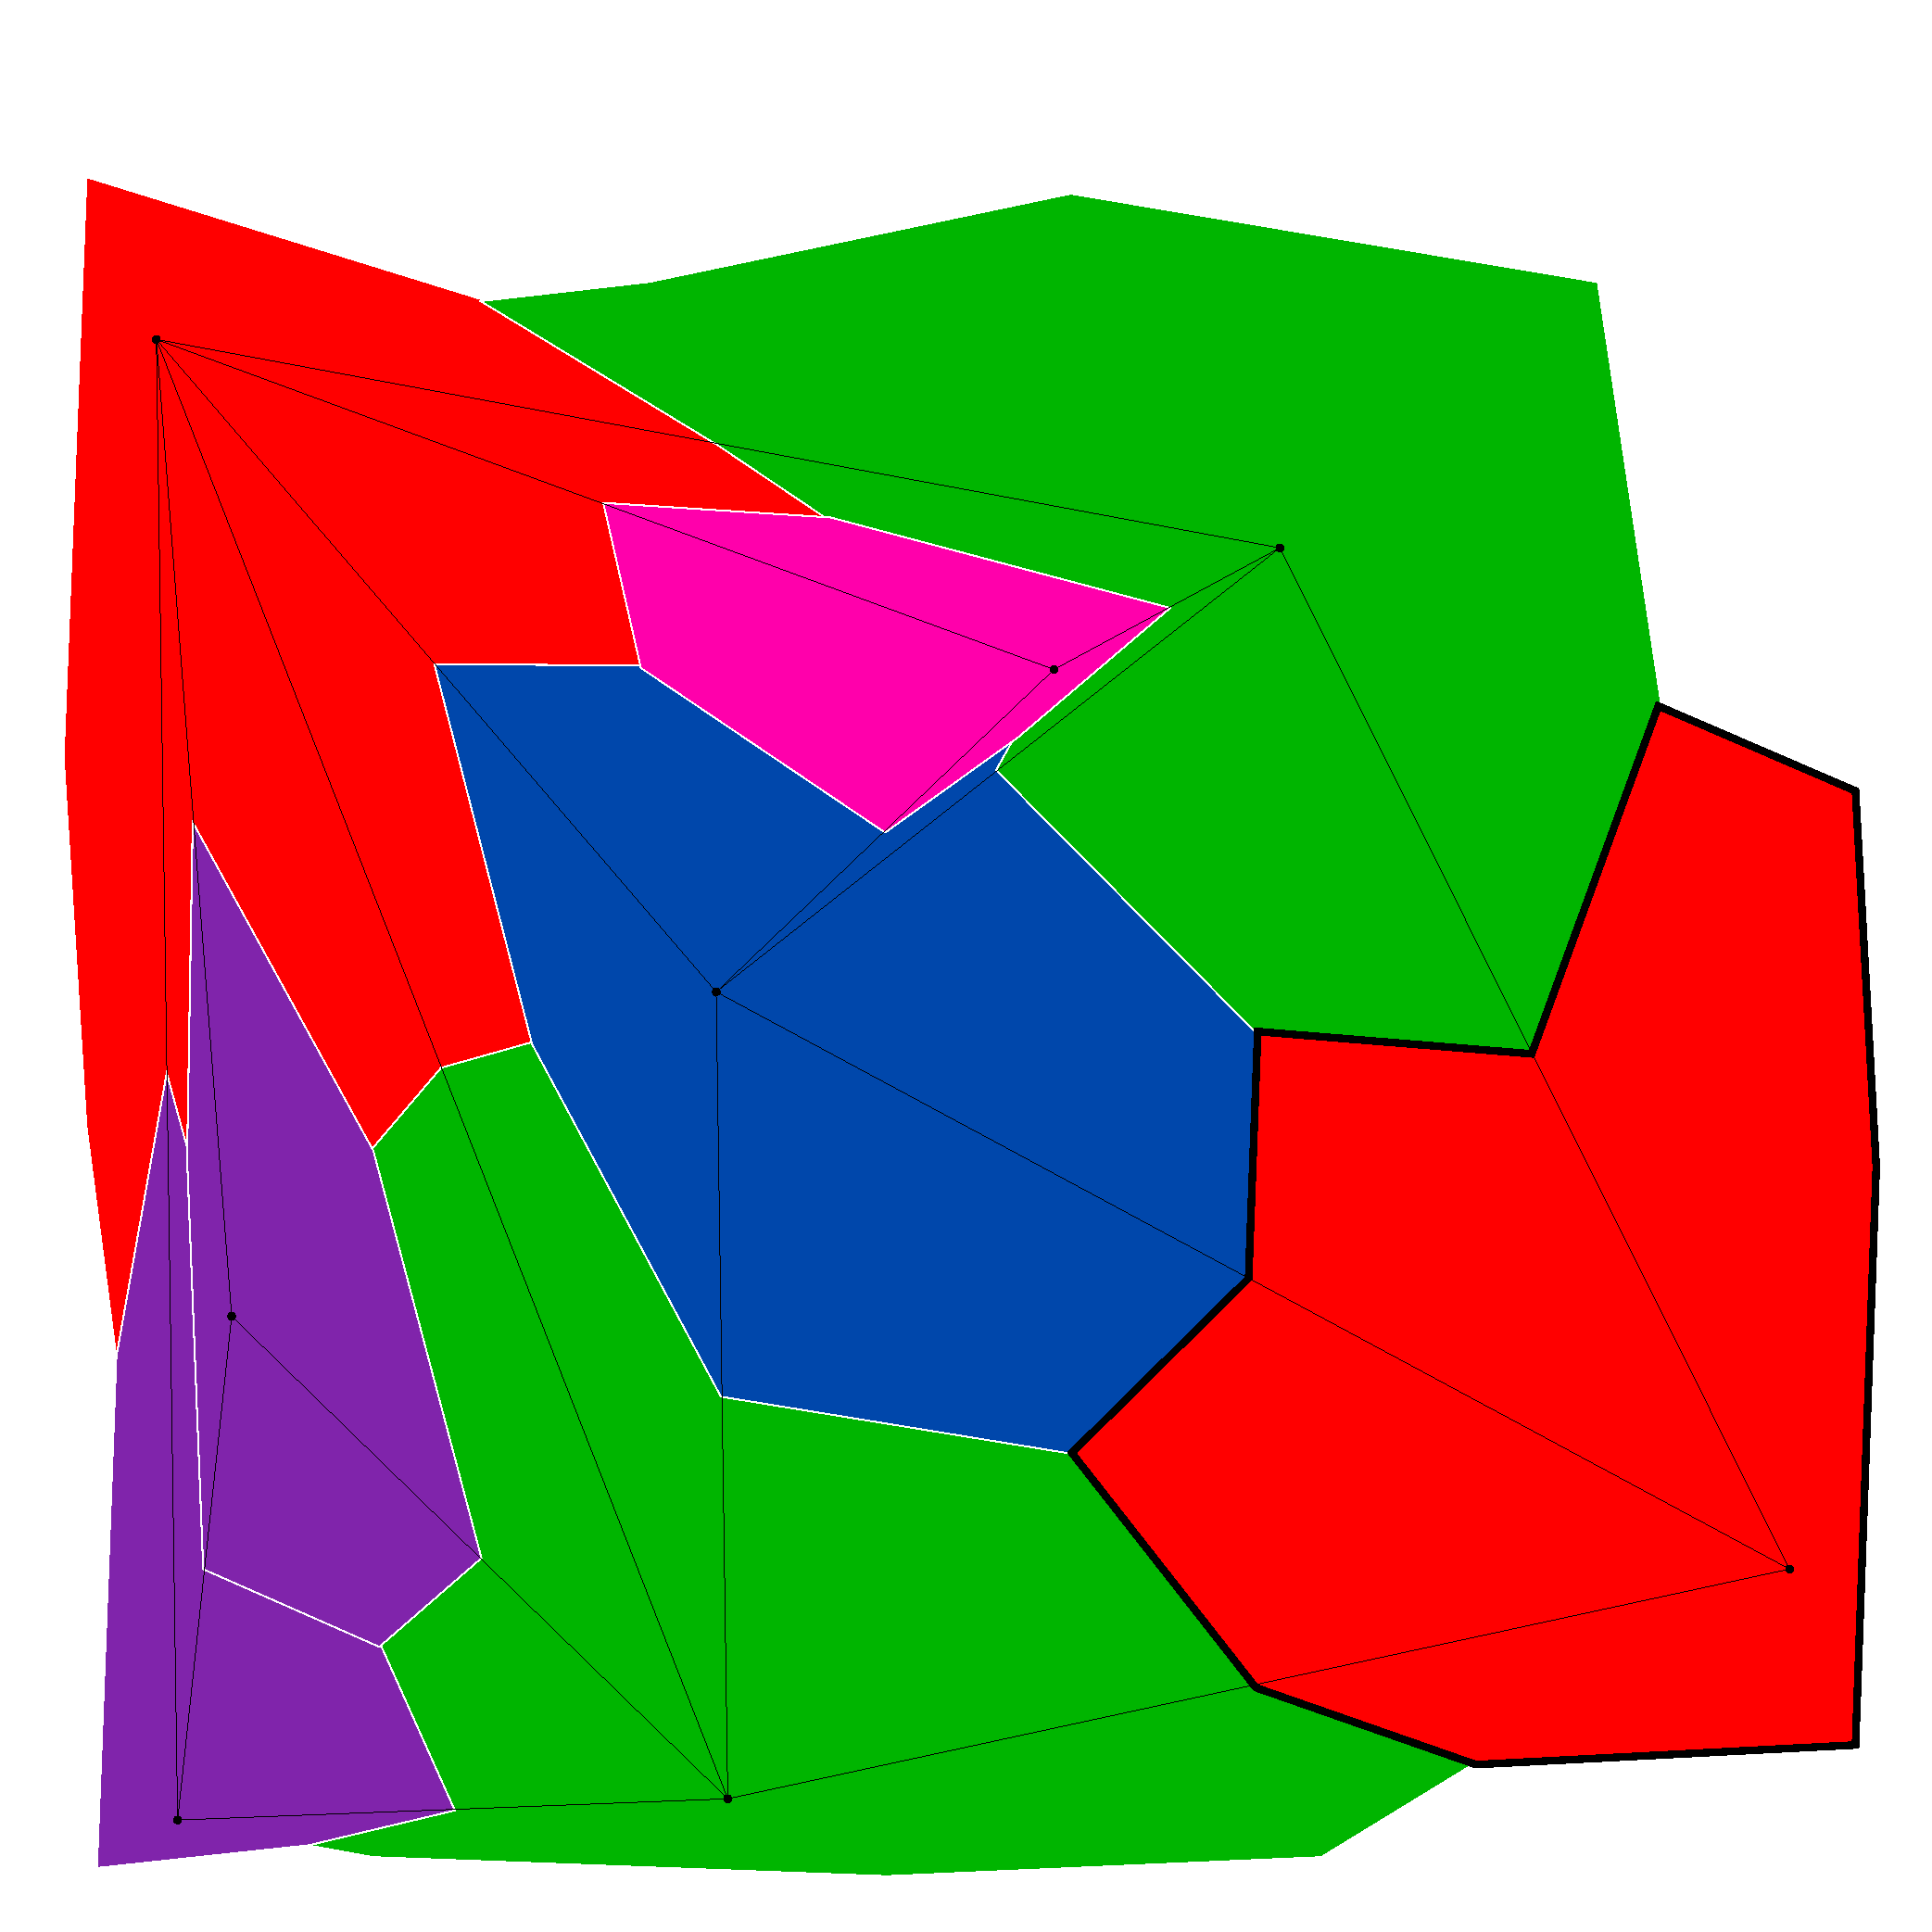
\includegraphics[width=\textwidth]{images/sequences/mac_backtracking/bt_mac_I00010}
				\caption{}
			\end{subfigure} \\
			
			\begin{subfigure}{0.18\textwidth}
				\centering
				\includegraphics[width=\textwidth]{images/sequences/mac_backtracking/bt_mac_I00012}
				\caption{}
				\label{high_c1}
			\end{subfigure}
			\;
			\begin{subfigure}{0.18\textwidth}
				\centering
				\includegraphics[width=\textwidth]{images/sequences/mac_backtracking/bt_mac_I00014}
				\caption{}
				\label{high_c2}
			\end{subfigure}
			\;
			\begin{subfigure}{0.18\textwidth}
				\centering
				\includegraphics[width=\textwidth]{images/sequences/mac_backtracking/bt_mac_I00016}
				\caption{}
				\label{high_c3}
			\end{subfigure}
			\;
			\begin{subfigure}{0.18\textwidth}
				\centering
				\includegraphics[width=\textwidth]{images/sequences/mac_backtracking/bt_mac_I00017}
				\caption{}
				\label{high_c4}
			\end{subfigure}
			\;
			\begin{subfigure}{0.18\textwidth}
				\centering
				\includegraphics[width=\textwidth]{images/sequences/mac_backtracking/bt_mac_I00018}
				\caption{}
				\label{high_c5}
			\end{subfigure}
	
			\caption{The map coloring example from Figure \ref{simple_ex} using backtracking with constraint propagation.}
			\label{mac_example}
		\end{figure}
		
		To see how backtracking with constraint propagation improves upon the idea of backtracking with forward checking, we turn one last time to the example introduced in Section \ref{simpe_desc}. Start by comparing Figures \ref{forward_example} and \ref{mac_example}. Notice how panels up to \ref{high_f1} and \ref{high_c1} are precisely the same. Backtracking with forward checking and backtracking with constraint propagation haven't diverged up to this point since this is a small graph. The first change occurs when vertex (g) is assigned the color blue in panel \ref{high_c2}. In the forward checking example, this reduces the color possibilities on vertex (j) to pink in panel \ref{high_f2}. But in the constraint propagation example it propagates this information to vertex (h) and (i) in panel \ref{high_c2}, reducing them to blue and null, respectively. Since constraint propagation noticed this error two steps earlier than forward checking, it is able to quickly recurse back in panels \ref{high_c3} and \ref{high_c4} far enough to change vertex (e) to blue in panel \ref{high_c5}. This change allows the solution to be found almost immediately, as the next choice for vertex (f) is green, which constrains vertex (g) to pink, (j) to blue, (h) to pink, and (i) to red.
		
		While the example above may seem only incrementally better than forward checking, as we will see in Section \ref{comparisons}, constraint propagation with MAC adds another large improvement to the backtracking algorithm from forward checking. This is because this algorithm can prune off large sections of the search tree by performing a search of the local neighborhood at each recursive backtracking step.
		
		In our implementation of backtracking with constraint propagation we used the algorithm AC-3 introduced by Mackworth in 1977 \cite{mackworth}. This algorithm is described in depth by Figure 6.3 of Russel and Norvig \cite{ai}.  At the heart of AC-3 is a function denoted \textsc{Revise}. The task of \textsc{Revise} is to loop through the possible colors $i$ in one vertex and make sure that it is consistent with all the possible colors $j$ in a neighboring vertex. If any $i$ is incompatible with all of $j$, it is deleted from the list of possible colors, and \textsc{Revise} returns \texttt{true}, indicating that the domian $i$ has been reduced. Otherwise, \textsc{Revise} returns \texttt{false} since $i$ remained unchanged.
		
		AC-3 uses a queue of remaining vertices and the function \textsc{Revise} to propagate constraints across the whole graph, while simultaneously maintaining arc consistency. For each vertex in the queue AC-3 calls \textsc{Revise} to see if the vertex provided any new information. If \textsc{Revise} returns \texttt{true}, AC-3 first checks if the domain $i$ is zero, if so, AC-3 returns \texttt{false}, signifying an arc consistency violation. If the domain of $i$ is nonzero, AC-3 propagates the information obtained through \textsc{Revise} by adding the vertex's neighbors to the queue. AC-3 continues until its queue is empty and returns \texttt{true}.
		
		Similar to backtracking with forward checking, backtracking with constraint propagation makes a small modification to the function \textsc{Backtrack}, but instead of calling \texttt{forward\_check()} before the next recursive call, we will ensure that AC-3 evaluates to \texttt{true} before the next recursive call to \textsc{Backtrack}.
	\subsection{Experimental Approach}
	
		Again, the experimental approach for this backtracking algorithm does not differ greatly from the previous two versions of backtracking. We do note, however, that constraint propagation and MAC do have an increased read and write overhead when compared to forward checking and simple backtracking. Since constraint propagation introduces even more overhead than forward checking on top of backtracking, in Section \ref{comparisons} we will see at what point, if ever, constraint propagation outpaces backtracking.
	
	\subsection{Results}
	
		\begin{figure}[h!]
			\centering
			\includegraphics[width=0.6\textwidth]{../results_5/backtracking_mac/bt_mac_performance}
			\caption{Logarithmic plot describing the performance of the backtracking with constraint propagation algorithm vs. the number of vertices. The shaded regions represent the minimum and maximum values of each quantity.}
			\label{mac_results}
		\end{figure}
		
		Compared to simple backtracking, backtracking with constraint propagation, displayed in Figure \ref{mac_results}, has a tremendous amount of read/write overhead per recursive call. At $N=10$, there were at least an order of magnitude more reads than recursive calls, but by $N=100$, there were almost two orders of magnitude more reads than recursive calls. This behavior indicates that the overhead of backtracking with constraint propagation is even larger than that of forward checking. This is to be expected, because AC-3 could potential visit every vertex in the graph for each recursive call.
		
		As with all the algorithms in this document, backtracking with constraint propagation behaves exponentially with increasing $N$. From this plot however, we can see that it certainly seems like backtracking with constraint propagation has a smaller slope on the logarithmic plot than the other two backtracking algorithms.
	
\section{Genetic Algorithm}

	\subsection{Implementation}
	Local search using a genetic algorithm involves a process similar to evolution to produce an individual that maximizes a fitness function. Since genetic algorithms are an abstraction of biological evolution, they involve some of the classic mechanisms seen in the natural world such as crossover, mutation, and survival of the fittest\cite{genetic}.
	
	The genetic algorithm begins with a population of randomly generated individuals. A selection process chooses which individuals to use for reproduction, which are weighted by their score generated the fitness function. The individuals are recombined by cross-over and the resulting individuals may be mutated depending on a small probability.
	
	To apply the genetic algorithm to the GCP we started with the genetic algorithm described in Russel and Norvig Section 4.1\cite{ai} and implemented each feature in accordance with the GCP. Our initial population consisted of $N$ randomly colored graphs. It was hard to determine what population size was the best, but it was clear that the optimal population size was related to the size of each graph and that larger graphs needed larger populations in general. $N$ was a logical number to try and it seemed to work fairly well.
	
	
	
	To select individuals for crossover we used tournament selection, in which two individuals were randomly selected and the one with the best fitness score  proceeded to crossover. Naturally, two tournaments were needed to get the two individuals required for crossover. In this scheme an individual could be chosen zero, one, or multiple times to participate in tournaments.
	
	The fitness function used to calculate the fitness score was essentially a penalty function because only the total number of conflicts in each individual was used to calculate the fitness score. Since this score reflected how many neighboring vertices shared colors, a large score was considered less fit and a score of zero indicated that a solution was found. 
	
	The crossover algorithm consisted of random single point crossover. To achieve this we chose a random point in each graph and swapped colors up to that point. The crossover example in Figure \ref{cross_example} looks like multi-point crossover because the vertices of the graph are unordered when crossover is performed.
	
	
	
	
	
	
	\begin{figure}[h!]
		\centering
		\begin{subfigure}{0.18\textwidth}
			\centering
			\includegraphics[width=\textwidth]{images/sequences/genetic/genetic_I00001}
			\caption{}
			
		\end{subfigure}
		\;
		\begin{subfigure}{0.18\textwidth}
			\centering
			\includegraphics[width=\textwidth]{images/sequences/genetic/genetic_I00002}
			\caption{}
			
		\end{subfigure}
		\;
		\\
		\begin{subfigure}{0.18\textwidth}
			\centering
			\includegraphics[width=\textwidth]{images/sequences/genetic/genetic_I00003}
			\caption{}
			
		\end{subfigure}
		\;		
		\begin{subfigure}{0.18\textwidth}
			\centering
			\includegraphics[width=\textwidth]{images/sequences/genetic/genetic_I00004}
			\caption{}
			
		\end{subfigure}
		
		\caption{Simple example of crossover where (a) and (b) are the parents and (c) and (d) are the offspring.}
		\label{cross_example}
	\end{figure}
	
	After crossover, we immediately mutated each individual which consisted of selecting each vertex and randomly changing it depending on a mutation rate defined as $1/N$. This mutation rate was chosen because it seemed to minimize the number of iterations to find a solution. This number proved to be very specific and any deviation would negatively affect the performance of the algorithm considerably. 
	
	Once we had the new individuals, we inserted them into the new population. We used pure insertion, meaning that each generation was composed entirely of new individuals produced by crossover. This was later understood to be a poor choice, but it did work for this application. 
	
	This process of selection, crossover, mutation, and reinsertion was repeated until an individual with zero conflicts was found or a predefined limit on the number of generations allowed was reached. In Figure \ref{genetic_flow} a flow graph showing the general flow of our genetic algorithm. It can be seen that the population is initialized outside of the main loop. 
	
	\begin{figure}[h!]
		\centering
		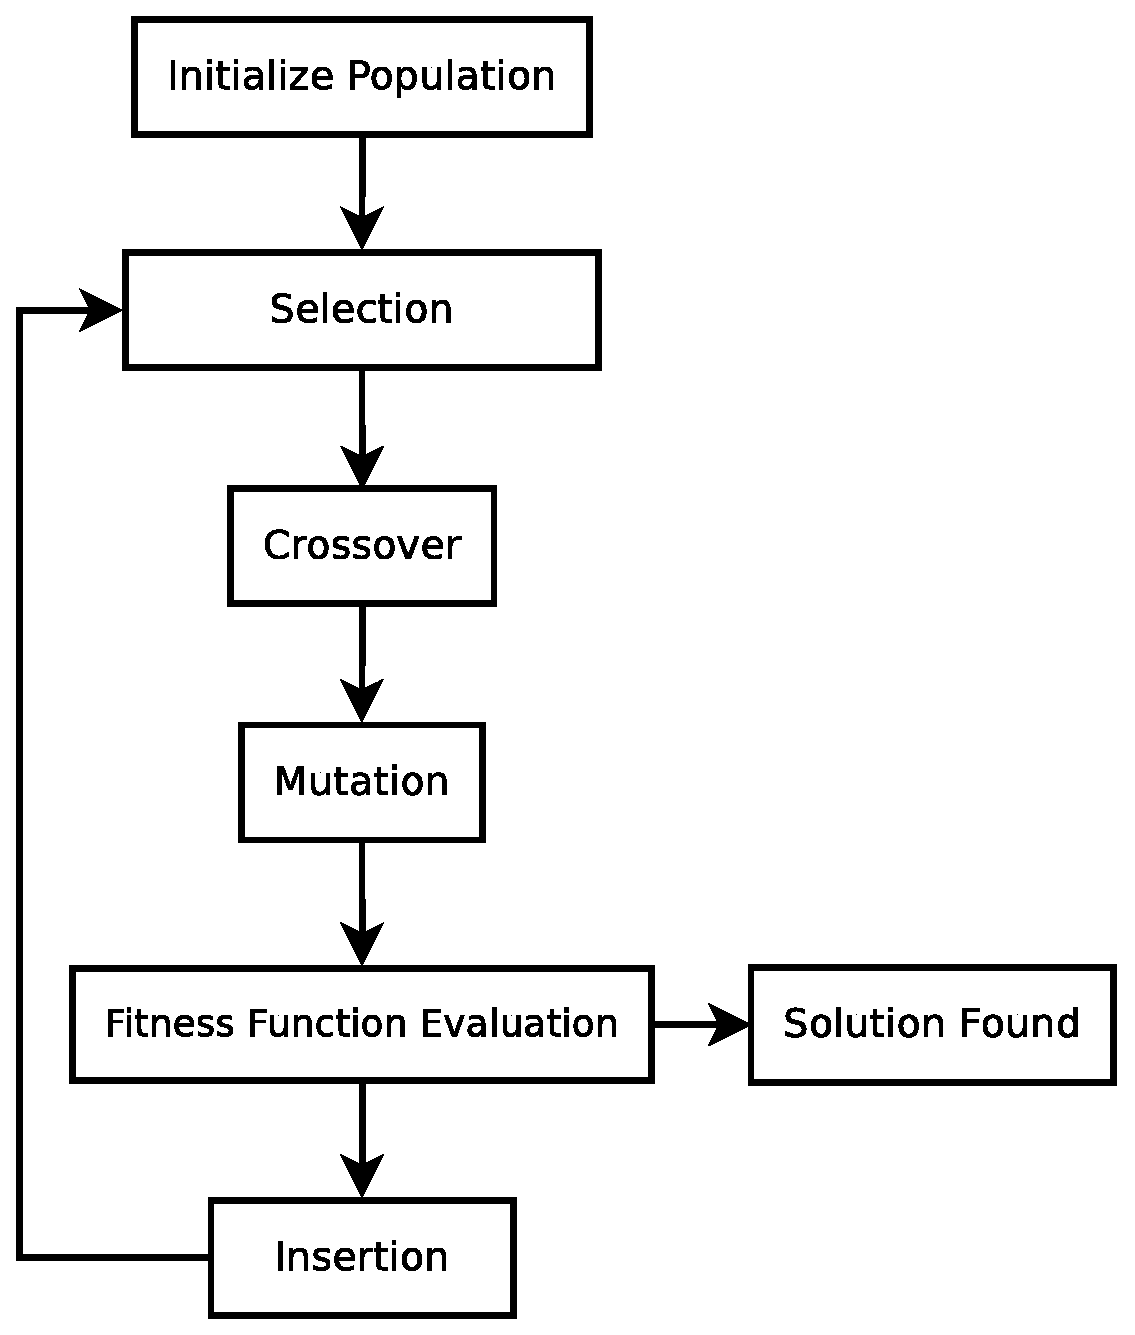
\includegraphics[width=0.3\textwidth]{images/genetic_flo}
		\caption{Flow graph of our genetic algorithm.}
		\label{genetic_flow}
	\end{figure}
	
	\subsection{Experimental Approach}
	To gauge the performance of the algorithm we will run the algorithm on graph sizes $N = (10, 20, ..., 100)$ with 20 runs of each different graph size. The metrics that will be used are number of generations, number of writes, and number of reads.
	
	The most obvious metric to use was number of generations because it tells us how many steps it took to find a solution. It was used to see how performance changed as $N$ increased and to compare the relative difficulty of graphs of the same size. Another added benefit of this metric was that it was used to find the optimal population size and mutation rate. The drawback of this metric was that it did not take into account the increased computation needed for larger graphs.
	
	One way we accounted for the increased computation time needed for larger graphs was to count the number of times we check the color of a graph vertex. This scaled with the size of the graph for two reasons. One was that each time we checked the fitness of a graph we had to read each nodes color and, as the graph got bigger, more nodes had to be read. The other reason is that, since our population is of size $N$, we have to check more graphs as the population size grows. We called this metric \texttt{num\_reads}
	
	The other way we accounted for the increased computation time needed for larger graphs was to count the number of times we change the color of a graph vertex. This metric scaled with the size of the graph for the same reasons as number of reads.
	
	\subsection{Results}
	\begin{figure}[h!]
		\centering
		\includegraphics[width=0.6\textwidth]{../results_5/genetic/genetic_performance}
		\caption{Logarithmic plot describing the performance of the genetic algorithm vs. the number of vertices. The shaded regions represent the minimum and maximum values of each quantity.}
		\label{genetic_Performance}
	\end{figure}
	
	Figure \ref{genetic_Performance} shows our metrics on a logarithmic plot. There are several points of interest on this graph. The first is how the number of generations increase as $N$ increases. We can deduce from the slope of the lines that this algorithm runs in exponential time, although it is still much faster than a brute force approach. We can further deduce that the number of generations increases at $\mathcal{O} (e^{Na})$ where $a$ represents the slope of the line in a logarithmic plot. By deduction we can see that  $a<1$.
	
	The other points of interest are the number of reads and writes. It can be seen that the slope of the line is a little more steep than the number of generations. This is as expected because the population size increases as $N$ increases and therefore causes the number of reads and writes to grow. Even with these setbacks, read and write still managed to run in approximately  $\mathcal{O} (e^{Nb})$, where $b$ represents the slope of the line in a logarithmic plot. By deduction we can see that the slope is greater than that of the number of generations and therefore $a<b$. Additionally we can see that the slope is less than one so we can further constrict b to $a<b<1$. 
\section{Comparing Algorithm Performance}
	\label{comparisons}
	
	\subsection{Experimental Approach}
	
	As described in the preceding sections, the number of vertex reads and number of vertex writes were our main metrics for comparing algorithm performance. Under these metrics, all calculations performed by each algorithm were assumed to be constant between subsequent reads and writes. This assumption is obviously untrue, but tests on our algorithm showed that this assumption was certainly reasonable because the rates (reads/s or writes/s) for each algorithm differed by only a constant factor for all $N$. This constant factor was large for some algorithms but was always dwarfed by the exponential time-complexity of the graph coloring problem.
	
	Though we are confident that measuring vertex reads and writes is an accurate metric of algorithm performance, to provide a counter-example we also measured the time required by each algorithm to find a solution to the GCP. Measuring algorithm performance using execution time is generally considered to be tenuous, as many things can affect a program's runtime, such as the hardware its being executed on, what other programs are being run at the same time, etc. We have noted these issues and have made every effort to make this test more accurate. These efforts include running all of the algorithms on the same machine to negate hardware differences, running only one algorithm at a time to eliminate the possibility of a memory bottleneck, and ensuring that no other programs are running on the machine during our tests. Another contentious facet of execution time metrics, is that one algorithm may simply be more optimized than another, and comparing a poor implementation of min-conflicts against a good implementation of backtracking, for example, would not be a very accurate test. This issue is much harder to mitigate and its effects will be ignored for this analysis.

	\subsection{Results}
	
		\begin{figure}[h!]
			\centering
			\begin{subfigure}{0.49\textwidth}
				\centering
				\includegraphics[width=\textwidth]{../results_5/comparing_read_performance}
				\caption{Average number of vertex reads for each algorithm.}
			\end{subfigure}
			\;
			\begin{subfigure}{0.49\textwidth}
				\centering
				\includegraphics[width=\textwidth]{../results_5/comparing_write_performance}
				\caption{Average number of vertex writes for each algorithm.}
			\end{subfigure} 
			\\
			\begin{subfigure}{0.49\textwidth}
				\centering
				\includegraphics[width=\textwidth]{../results_5/comparing_time_performance}
				\caption{Average amount of time elapsed for each algorithm.}
			\end{subfigure}
			\;
			\begin{subfigure}{0.49\textwidth}
				\centering
				\includegraphics[width=\textwidth]{../results_5/comparing_num_saturated}
				\caption{Number of trials that reached the computation limit.}
				\label{comp_limit}
			\end{subfigure}
			\caption{Logarithmic plots comparing the performance of the five different GCP algorithms against four different measurements. Shaded regions represent the maximum and minimum values.}
			\label{results}
		\end{figure}
		
		In general, the minimum conflicts was the fastest algorithm for large $N$, but it was by no means the clear winner as we expected. In terms of reads, min-conflicts was just as fast as backtracking with MAC up until $N=100$, where it gained a marginal lead, ending up in first place at an average of between 10 and 100 million reads per solution. In terms of writes, it was obvious that minimum conflicts was growing out the slowest out of any algorithm from the start, completing an $N=100$ graph in over two orders of magnitude fewer writes than the second place algorithm, backtracking with MAC. Surprisingly, min-conflicts was not the fastest algorithm in terms of elapsed time until $N=100$. We are not sure how to explain this phenomenon, but it is an indication that measuring vertex reads and writes may not be the most appropriate measurement.
		
		Simple backtracking began by being just as fast as the other two variations of backtrack and min-conflicts, but grew at a rate faster than any of the other algorithms, finishing in the same place as the genetic algorithm. However, the average number of reads and writes is misleading in this case. Notice how the maximum and minimum values of simple backtracking span the range of almost every other algorithm combined in all three graphs in Figure \ref{results}. This indicates that simple backtracking is sometimes just as fast as the min-conflicts and backtracking with MAC, but it can also be much slower, at least five orders of magnitude slower in terms of reads at $N=100$. Furthermore, we also note from Figure \ref{comp_limit} that simple backtracking hit the computation limit in 2 out of 20 runs at $N=100$. This implies that the actual average value of reads, writes, and elapsed time would be larger if this limit had not been reached. Interestingly enough, simple backtracking is the fastest out of any algorithm for the $N=10$ case in terms of elapsed time, indicating that it requires the least overhead of any algorithm.
		
		Backtracking with forward checking was a huge improvement on simple backtracking, finishing an order of magnitude faster in reads, writes and elapsed time at $N=100$. However, forward checking was also slower than the two fastest algorithms, finishing more than two orders of magnitude behind backtracking with MAC at $N=100$. Forward checking was the fastest algorithm in terms of elapsed time between $N=20$ and $N=30$. This region is where the additional overhead from constraint propagation is unnecessary, but the raw speed from simple backtracking is not enough to solve the problems quickly.
	
		Almost as fast as min-conflicts, was backtracking with MAC. In terms of reads, min-conflicts and backtracking with MAC seem to growing nearly at the same rate, only diverging at the last point. It would be interesting to see if min-conflicts could retain its lead for larger values of $N$. In terms of vertex writes, it seems that backtracking with MAC cannot compete with min-conflicts, growing at a much faster rate to finish two orders of magnitude slower than min-conflicts at $N=100$. But, just like the other backtracking algorithms, backtracking with MAC is initially faster than min-conflicts in terms of elapsed time. Backtracking with MAC has more overhead than the other two backtracking algorithms, so it only starts to gain an advantage in terms of elapsed time after $N=40$. It holds onto this lead until $N=100$, where it is finally beat by min-conflicts.
		
		The genetic algorithm had much more overhead in terms of reads and writes for low values of $N$ under all three metrics. Fortunately, this overhead payed off for larger values of $N$, as the genetic algorithm grew slower than most of the other algorithms, finishing in the same amount of reads and writes as simple backtracking at $N=100$. In terms of elapsed time, the genetic algorithm did even better, finishing in the middle of the pack behind min-conflicts and backtracking with MAC. From the trends in all three plots, it seems reasonable to think that the genetic algorithm would eventually become more efficient than all of the backtracking algorithms as $N$ increased beyond 100. It is harder to determine if the genetic algorithm would ever be faster than minimum conflicts. From the read/write plots, it would seem that the time-complexity of the genetic algorithm is growing faster than the time-complexity of min-conflicts. However, from the elapsed-time plot, it seems that the time complexity of the genetic algorithm is growing slower than min-conflicts, so obviously more research would be required.
	
\section{Summary}

	\begin{figure}[h!]
		\centering
		\includegraphics[width=0.4\textwidth]{images/colored_example}
		\caption{Example of a fully colored, 100 vertex graph produced by backtracking with constraint propagation.}
	\end{figure}
	
	In this paper, we have studied the performance of minimum conflicts, simple backtracking, backtracking with forward checking, backtracking with constraint propagation, and a genetic algorithm on the graph coloring problem. To determine performance, we developed an implementation of each algorithm in \texttt{C++}. Each algorithm was run many times on graphs with varying number of vertices to explore the time-complexity of each algorithm. 
	
	
	In general, all of the algorithms were very successful at solving this problem, every algorithm could reliably find solutions for most problems in a reasonable amount of time. However, some algorithms were undeniably more efficient at solving the graph coloring problem, namely min-conflicts and backtracking with constraint propagation. These algorithms were much faster than simple backtracking and backtracking with forward checking, completing solutions to the GCP in over an order of magnitude fewer steps.
	
	Of special note is the genetic algorithm. This algorithm had the most overhead of any of algorithms we tested. However, the leading-order time complexity of the genetic algorithm was comparable to that of backtracking with MAC and min-conflicts. Therefore, it may be that the genetic algorithm would eventually be more efficient than backtracking with MAC and min-conflicts if the number of vertices was large enough. More research will be needed to answer this question.
	
	We would also like to mention that the variation in performance of the five algorithms was very large. The results above exhibit a large dependence on the graph coloring problem being solved, and a different dataset may produce vastly different results. However, in our experience each of the five algorithms usually have the same performance relative to one another, e.g. we have never seen a dataset where min-conflicts was slower than the rest of the algorithms.

	

	\pagebreak


	%\bibliographystyle{apj}
	\bibliographystyle{unsrt}
	
	\bibliography{sources}
\end{document}
